% Options for packages loaded elsewhere
\PassOptionsToPackage{unicode}{hyperref}
\PassOptionsToPackage{hyphens}{url}
%
\documentclass[
]{article}
\usepackage{amsmath,amssymb}
\usepackage{lmodern}
\usepackage{iftex}
\ifPDFTeX
  \usepackage[T1]{fontenc}
  \usepackage[utf8]{inputenc}
  \usepackage{textcomp} % provide euro and other symbols
\else % if luatex or xetex
  \usepackage{unicode-math}
  \defaultfontfeatures{Scale=MatchLowercase}
  \defaultfontfeatures[\rmfamily]{Ligatures=TeX,Scale=1}
\fi
% Use upquote if available, for straight quotes in verbatim environments
\IfFileExists{upquote.sty}{\usepackage{upquote}}{}
\IfFileExists{microtype.sty}{% use microtype if available
  \usepackage[]{microtype}
  \UseMicrotypeSet[protrusion]{basicmath} % disable protrusion for tt fonts
}{}
\makeatletter
\@ifundefined{KOMAClassName}{% if non-KOMA class
  \IfFileExists{parskip.sty}{%
    \usepackage{parskip}
  }{% else
    \setlength{\parindent}{0pt}
    \setlength{\parskip}{6pt plus 2pt minus 1pt}}
}{% if KOMA class
  \KOMAoptions{parskip=half}}
\makeatother
\usepackage{xcolor}
\usepackage[margin=1in]{geometry}
\usepackage{color}
\usepackage{fancyvrb}
\newcommand{\VerbBar}{|}
\newcommand{\VERB}{\Verb[commandchars=\\\{\}]}
\DefineVerbatimEnvironment{Highlighting}{Verbatim}{commandchars=\\\{\}}
% Add ',fontsize=\small' for more characters per line
\usepackage{framed}
\definecolor{shadecolor}{RGB}{248,248,248}
\newenvironment{Shaded}{\begin{snugshade}}{\end{snugshade}}
\newcommand{\AlertTok}[1]{\textcolor[rgb]{0.94,0.16,0.16}{#1}}
\newcommand{\AnnotationTok}[1]{\textcolor[rgb]{0.56,0.35,0.01}{\textbf{\textit{#1}}}}
\newcommand{\AttributeTok}[1]{\textcolor[rgb]{0.77,0.63,0.00}{#1}}
\newcommand{\BaseNTok}[1]{\textcolor[rgb]{0.00,0.00,0.81}{#1}}
\newcommand{\BuiltInTok}[1]{#1}
\newcommand{\CharTok}[1]{\textcolor[rgb]{0.31,0.60,0.02}{#1}}
\newcommand{\CommentTok}[1]{\textcolor[rgb]{0.56,0.35,0.01}{\textit{#1}}}
\newcommand{\CommentVarTok}[1]{\textcolor[rgb]{0.56,0.35,0.01}{\textbf{\textit{#1}}}}
\newcommand{\ConstantTok}[1]{\textcolor[rgb]{0.00,0.00,0.00}{#1}}
\newcommand{\ControlFlowTok}[1]{\textcolor[rgb]{0.13,0.29,0.53}{\textbf{#1}}}
\newcommand{\DataTypeTok}[1]{\textcolor[rgb]{0.13,0.29,0.53}{#1}}
\newcommand{\DecValTok}[1]{\textcolor[rgb]{0.00,0.00,0.81}{#1}}
\newcommand{\DocumentationTok}[1]{\textcolor[rgb]{0.56,0.35,0.01}{\textbf{\textit{#1}}}}
\newcommand{\ErrorTok}[1]{\textcolor[rgb]{0.64,0.00,0.00}{\textbf{#1}}}
\newcommand{\ExtensionTok}[1]{#1}
\newcommand{\FloatTok}[1]{\textcolor[rgb]{0.00,0.00,0.81}{#1}}
\newcommand{\FunctionTok}[1]{\textcolor[rgb]{0.00,0.00,0.00}{#1}}
\newcommand{\ImportTok}[1]{#1}
\newcommand{\InformationTok}[1]{\textcolor[rgb]{0.56,0.35,0.01}{\textbf{\textit{#1}}}}
\newcommand{\KeywordTok}[1]{\textcolor[rgb]{0.13,0.29,0.53}{\textbf{#1}}}
\newcommand{\NormalTok}[1]{#1}
\newcommand{\OperatorTok}[1]{\textcolor[rgb]{0.81,0.36,0.00}{\textbf{#1}}}
\newcommand{\OtherTok}[1]{\textcolor[rgb]{0.56,0.35,0.01}{#1}}
\newcommand{\PreprocessorTok}[1]{\textcolor[rgb]{0.56,0.35,0.01}{\textit{#1}}}
\newcommand{\RegionMarkerTok}[1]{#1}
\newcommand{\SpecialCharTok}[1]{\textcolor[rgb]{0.00,0.00,0.00}{#1}}
\newcommand{\SpecialStringTok}[1]{\textcolor[rgb]{0.31,0.60,0.02}{#1}}
\newcommand{\StringTok}[1]{\textcolor[rgb]{0.31,0.60,0.02}{#1}}
\newcommand{\VariableTok}[1]{\textcolor[rgb]{0.00,0.00,0.00}{#1}}
\newcommand{\VerbatimStringTok}[1]{\textcolor[rgb]{0.31,0.60,0.02}{#1}}
\newcommand{\WarningTok}[1]{\textcolor[rgb]{0.56,0.35,0.01}{\textbf{\textit{#1}}}}
\usepackage{longtable,booktabs,array}
\usepackage{calc} % for calculating minipage widths
% Correct order of tables after \paragraph or \subparagraph
\usepackage{etoolbox}
\makeatletter
\patchcmd\longtable{\par}{\if@noskipsec\mbox{}\fi\par}{}{}
\makeatother
% Allow footnotes in longtable head/foot
\IfFileExists{footnotehyper.sty}{\usepackage{footnotehyper}}{\usepackage{footnote}}
\makesavenoteenv{longtable}
\usepackage{graphicx}
\makeatletter
\def\maxwidth{\ifdim\Gin@nat@width>\linewidth\linewidth\else\Gin@nat@width\fi}
\def\maxheight{\ifdim\Gin@nat@height>\textheight\textheight\else\Gin@nat@height\fi}
\makeatother
% Scale images if necessary, so that they will not overflow the page
% margins by default, and it is still possible to overwrite the defaults
% using explicit options in \includegraphics[width, height, ...]{}
\setkeys{Gin}{width=\maxwidth,height=\maxheight,keepaspectratio}
% Set default figure placement to htbp
\makeatletter
\def\fps@figure{htbp}
\makeatother
\setlength{\emergencystretch}{3em} % prevent overfull lines
\providecommand{\tightlist}{%
  \setlength{\itemsep}{0pt}\setlength{\parskip}{0pt}}
\setcounter{secnumdepth}{-\maxdimen} % remove section numbering
\ifLuaTeX
  \usepackage{selnolig}  % disable illegal ligatures
\fi
\IfFileExists{bookmark.sty}{\usepackage{bookmark}}{\usepackage{hyperref}}
\IfFileExists{xurl.sty}{\usepackage{xurl}}{} % add URL line breaks if available
\urlstyle{same} % disable monospaced font for URLs
\hypersetup{
  pdftitle={Reporting with RMarkdown},
  pdfauthor={Joschka Schwarz},
  hidelinks,
  pdfcreator={LaTeX via pandoc}}

\title{Reporting with RMarkdown}
\author{Joschka Schwarz}
\date{9/15/2020}

\begin{document}
\maketitle

{
\setcounter{tocdepth}{2}
\tableofcontents
}
\hypertarget{rmarkdown}{%
\section{RMarkdown}\label{rmarkdown}}

\begin{quote}
Is amazing.
\end{quote}

\hypertarget{what-can-rmarkdown-be-used-for}{%
\subsection{What can RMarkdown be used
for?}\label{what-can-rmarkdown-be-used-for}}

\begin{enumerate}
\def\labelenumi{\arabic{enumi}.}
\tightlist
\item
  \href{https://bookdown.org/yihui/rmarkdown/html-document.html}{HTML
  Reports} \&
  \href{https://bookdown.org/yihui/rmarkdown/pdf-document.html}{PDF
  Reports}
\item
  \href{https://bookdown.org/yihui/rmarkdown/ioslides-presentation.html}{HTML
  Slide Decks} \&
  \href{https://bookdown.org/yihui/rmarkdown/powerpoint-presentation.html}{PowerPoint}
\item
  \href{https://rmarkdown.rstudio.com/flexdashboard/index.html}{Interactive
  Dashboards}
\item
  \href{https://bookdown.org/}{Books with \texttt{bookdown}}
\item
  \href{https://bookdown.org/yihui/blogdown/}{Websites with
  \texttt{blogdown}}
\end{enumerate}

\hypertarget{key-resources}{%
\subsection{Key Resources}\label{key-resources}}

\begin{itemize}
\item
  \href{https://rmarkdown.rstudio.com/index.html}{RMarkdown Website with
  Gallery}
\item
  Key Reference: \href{https://bookdown.org/yihui/rmarkdown/}{RMarkdown
  - The Definitive Guide}
\item
  PDF Printing Setup: \href{https://yihui.name/tinytex/}{tinytex}
\end{itemize}

\begin{Shaded}
\begin{Highlighting}[]
\CommentTok{\# PDF Knitting Setup: https://yihui.name/tinytex/ }
\CommentTok{\# install.packages("tintex")}
\CommentTok{\# tinytex::install\_tinytex()}
\end{Highlighting}
\end{Shaded}

\hypertarget{how-rmarkdown-works}{%
\section{How Rmarkdown Works}\label{how-rmarkdown-works}}

\hypertarget{header-1}{%
\section{Header 1}\label{header-1}}

\hypertarget{header-2}{%
\subsection{Header 2}\label{header-2}}

\hypertarget{header-3}{%
\subsubsection{Header 3}\label{header-3}}

\hypertarget{working-with-text}{%
\section{Working with Text}\label{working-with-text}}

Free-form text.

Make text \textbf{bold}.

Make text \emph{italics}.

Make text \textbf{\emph{bold + italics}}.

Talk about code - the \texttt{tidyverse} is awesome

\textbf{Unordered List:}

\begin{itemize}
\item
  Item 1
\item
  Item 2
\end{itemize}

\textbf{Ordered List:}

\begin{enumerate}
\def\labelenumi{\arabic{enumi}.}
\item
  First point
\item
  Second point
\item
  More points
\end{enumerate}

\hypertarget{tabset}{%
\section{Tabset}\label{tabset}}

\hypertarget{tab-1}{%
\subsection{Tab 1}\label{tab-1}}

This is Tab 1

\hypertarget{tab-2}{%
\subsection{Tab 2}\label{tab-2}}

This is Tab 2

\hypertarget{images}{%
\section{Images}\label{images}}

\begin{figure}
\centering

\includegraphics[width=1.04167in,height=\textheight]{img/logo_nit.png}
\caption{NIT Logo}
\end{figure}

\begin{figure}

{\centering 
\includegraphics[width=100px]{img/logo_nit} 

}

\caption{NIT Logo}\label{fig:unnamed-chunk-3}
\end{figure}

\hypertarget{code}{%
\section{Code}\label{code}}

Read in data and print to HTML. Notice effect of
\texttt{df\_print:\ paged} option for HTML.

\begin{itemize}
\item
  Try changing to \texttt{df\_print:\ default}, or \texttt{kable} or
  \texttt{tibble}. PDF prints normally.
\item
  Try changing \texttt{results\ =\ "hide"}.
\end{itemize}

\begin{Shaded}
\begin{Highlighting}[]
\CommentTok{\# Bike data}
\NormalTok{bikes\_tbl      }\OtherTok{\textless{}{-}} \FunctionTok{readRDS}\NormalTok{(}\StringTok{"01\_data/bikes\_tbl.rds"}\NormalTok{)}
\NormalTok{bikeshops\_tbl  }\OtherTok{\textless{}{-}} \FunctionTok{readRDS}\NormalTok{(}\StringTok{"01\_data/bikeshops\_tbl.rds"}\NormalTok{)}
\NormalTok{orderlines\_tbl }\OtherTok{\textless{}{-}} \FunctionTok{readRDS}\NormalTok{(}\StringTok{"01\_data/orderlines\_tbl.rds"}\NormalTok{)}

\NormalTok{bike\_orderlines\_tbl }\OtherTok{\textless{}{-}}\NormalTok{ orderlines\_tbl }\SpecialCharTok{\%\textgreater{}\%}
    \FunctionTok{left\_join}\NormalTok{(bikes\_tbl,     }\AttributeTok{by =} \FunctionTok{c}\NormalTok{(}\StringTok{"product\_id"} \OtherTok{=} \StringTok{"bike\_id"}\NormalTok{)) }\SpecialCharTok{\%\textgreater{}\%}
    \FunctionTok{left\_join}\NormalTok{(bikeshops\_tbl, }\AttributeTok{by =} \FunctionTok{c}\NormalTok{(}\StringTok{"customer\_id"} \OtherTok{=} \StringTok{"bikeshop\_id"}\NormalTok{)) }\SpecialCharTok{\%\textgreater{}\%}
    \FunctionTok{mutate}\NormalTok{(}\AttributeTok{total\_price =}\NormalTok{ price\_euro }\SpecialCharTok{*}\NormalTok{ quantity)}

\NormalTok{bike\_orderlines\_tbl}
\end{Highlighting}
\end{Shaded}

\begin{verbatim}
## # A tibble: 15,644 x 23
##    order_id order_line order_date          customer_id product_id quantity model
##       <dbl>      <dbl> <dttm>                    <dbl>      <dbl>    <dbl> <chr>
##  1        1          1 2015-01-07 00:00:00           2       2681        1 Spec~
##  2        1          2 2015-01-07 00:00:00           2       2411        1 Ulti~
##  3        2          1 2015-01-10 00:00:00          10       2629        1 Neur~
##  4        2          2 2015-01-10 00:00:00          10       2137        1 Spee~
##  5        3          1 2015-01-10 00:00:00           6       2367        1 Stit~
##  6        3          2 2015-01-10 00:00:00           6       1973        1 Road~
##  7        3          3 2015-01-10 00:00:00           6       2422        1 Spee~
##  8        3          4 2015-01-10 00:00:00           6       2655        1 Infl~
##  9        3          5 2015-01-10 00:00:00           6       2247        1 Torq~
## 10        4          1 2015-01-11 00:00:00          22       2408        1 Ulti~
## # i 15,634 more rows
## # i 16 more variables: year <dbl>, frame_material <chr>, weight <dbl>,
## #   price_euro <dbl>, category_1 <chr>, category_2 <chr>, category_3 <chr>,
## #   gender <chr>, description <chr>, url <chr>, name <chr>, city <chr>,
## #   state <chr>, lat <dbl>, lng <dbl>, total_price <dbl>
\end{verbatim}

We can do data manipulations too. Try changing the YAML
\texttt{code\_folding} option from \texttt{none} to \texttt{hide} to
\texttt{show}.

\begin{Shaded}
\begin{Highlighting}[]
\NormalTok{sales\_by\_category\_tbl }\OtherTok{\textless{}{-}}\NormalTok{ bike\_orderlines\_tbl }\SpecialCharTok{\%\textgreater{}\%}
\NormalTok{  dplyr}\SpecialCharTok{::}\FunctionTok{select}\NormalTok{(category\_2, category\_1, total\_price) }\SpecialCharTok{\%\textgreater{}\%}
  
  \FunctionTok{group\_by}\NormalTok{(category\_2, category\_1) }\SpecialCharTok{\%\textgreater{}\%}
  \FunctionTok{summarise}\NormalTok{(}\AttributeTok{total\_revenue =} \FunctionTok{sum}\NormalTok{(total\_price)) }\SpecialCharTok{\%\textgreater{}\%}
  \FunctionTok{ungroup}\NormalTok{() }\SpecialCharTok{\%\textgreater{}\%}
  
  \FunctionTok{arrange}\NormalTok{(}\FunctionTok{desc}\NormalTok{(total\_revenue)) }\SpecialCharTok{\%\textgreater{}\%}
  \FunctionTok{mutate}\NormalTok{(}\AttributeTok{category\_2 =} \FunctionTok{as\_factor}\NormalTok{(category\_2) }\SpecialCharTok{\%\textgreater{}\%} \FunctionTok{fct\_rev}\NormalTok{())}
\end{Highlighting}
\end{Shaded}

\hypertarget{plots}{%
\section{Plots}\label{plots}}

Plotting works as expected. Try changin:

\begin{itemize}
\item
  \texttt{out.height}, \texttt{out.width} and Knitting
\item
  Potential gotcha - Interactive plots (e.g.~\texttt{plotly}) will not
  display in PDF
\end{itemize}

\textbf{Static Plots:}

\begin{itemize}
\tightlist
\item
  Use \texttt{ggplot2}.
\end{itemize}

\begin{Shaded}
\begin{Highlighting}[]
\NormalTok{g }\OtherTok{\textless{}{-}}\NormalTok{ sales\_by\_category\_tbl }\SpecialCharTok{\%\textgreater{}\%}
  \FunctionTok{ggplot}\NormalTok{(}\FunctionTok{aes}\NormalTok{(category\_2, total\_revenue, }\AttributeTok{fill =}\NormalTok{ category\_1)) }\SpecialCharTok{+}
  
  \CommentTok{\# Geoms}
  \FunctionTok{geom\_col}\NormalTok{() }\SpecialCharTok{+}
  \FunctionTok{coord\_flip}\NormalTok{() }\SpecialCharTok{+}
  
  \CommentTok{\# Formatting}
  \FunctionTok{labs}\NormalTok{(}
    \AttributeTok{title =} \StringTok{"Total Revenue by Category"}\NormalTok{,}
    \AttributeTok{x =} \StringTok{""}\NormalTok{, }\AttributeTok{y =} \StringTok{""}\NormalTok{, }\AttributeTok{fill =} \StringTok{""}
\NormalTok{  )}

\NormalTok{g}
\end{Highlighting}
\end{Shaded}

\begin{figure}

{\centering 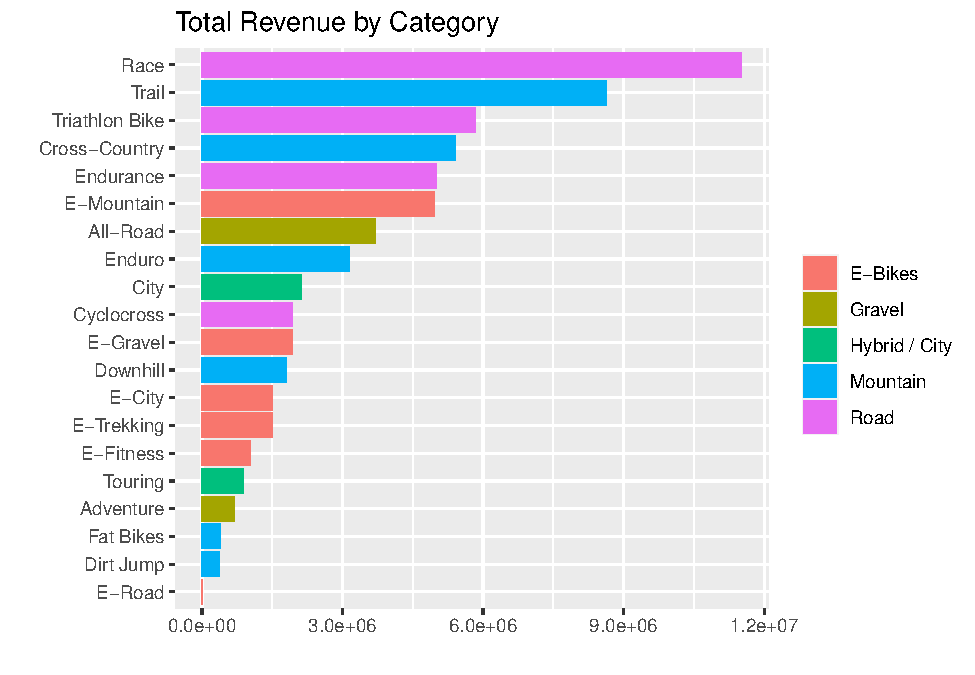
\includegraphics[height=600px]{reporting_rmarkdown_files/figure-latex/unnamed-chunk-6-1} 

}

\caption{Revenue by Category}\label{fig:unnamed-chunk-6}
\end{figure}

\textbf{Interactive plots:}

\begin{itemize}
\tightlist
\item
  Use \texttt{ggplotly()}.
\end{itemize}

\begin{Shaded}
\begin{Highlighting}[]
\CommentTok{\# ggplotly(g)}
\end{Highlighting}
\end{Shaded}

\hypertarget{tables}{%
\section{Tables}\label{tables}}

\textbf{Static Tables:}

\begin{itemize}
\tightlist
\item
  \texttt{knitr} package - \texttt{knitr::kable()} - Simple to use,
  great with PDF
\item
  \href{https://gt.rstudio.com/}{\texttt{gt} package} - Really good for
  static tables
\end{itemize}

\begin{Shaded}
\begin{Highlighting}[]
\NormalTok{table\_formatted\_tbl }\OtherTok{\textless{}{-}}\NormalTok{ sales\_by\_category\_tbl }\SpecialCharTok{\%\textgreater{}\%}
  \FunctionTok{rename\_all}\NormalTok{(}\AttributeTok{.funs =} \SpecialCharTok{\textasciitilde{}} \FunctionTok{str\_replace}\NormalTok{(., }\StringTok{"\_"}\NormalTok{, }\StringTok{" "}\NormalTok{) }\SpecialCharTok{\%\textgreater{}\%}
               \FunctionTok{str\_to\_title}\NormalTok{()) }

\NormalTok{table\_formatted\_tbl }\SpecialCharTok{\%\textgreater{}\%}\NormalTok{ knitr}\SpecialCharTok{::}\FunctionTok{kable}\NormalTok{()}
\end{Highlighting}
\end{Shaded}

\begin{longtable}[]{@{}llr@{}}
\toprule()
Category 2 & Category 1 & Total Revenue \\
\midrule()
\endhead
Race & Road & 11509156 \\
Trail & Mountain & 8644966 \\
Triathlon Bike & Road & 5831716 \\
Cross-Country & Mountain & 5421144 \\
Endurance & Road & 5013423 \\
E-Mountain & E-Bikes & 4962946 \\
All-Road & Gravel & 3697923 \\
Enduro & Mountain & 3156837 \\
City & Hybrid / City & 2115482 \\
Cyclocross & Road & 1940532 \\
E-Gravel & E-Bikes & 1936489 \\
Downhill & Mountain & 1803970 \\
E-City & E-Bikes & 1509096 \\
E-Trekking & E-Bikes & 1500894 \\
E-Fitness & E-Bikes & 1039996 \\
Touring & Hybrid / City & 877736 \\
Adventure & Gravel & 702007 \\
Fat Bikes & Mountain & 391654 \\
Dirt Jump & Mountain & 371922 \\
E-Road & E-Bikes & 2919 \\
\bottomrule()
\end{longtable}

\textbf{Dynamic Tables:}

\begin{itemize}
\tightlist
\item
  Can print tables without additional formatting in HTML with the
  \texttt{df\_print:\ paged} option in YAML
\item
  Potential Gotcha: Note that this will not print with format in PDF
\end{itemize}

\begin{Shaded}
\begin{Highlighting}[]
\NormalTok{table\_formatted\_tbl}
\end{Highlighting}
\end{Shaded}

\begin{verbatim}
## # A tibble: 20 x 3
##    `Category 2`   `Category 1`  `Total Revenue`
##    <fct>          <chr>                   <dbl>
##  1 Race           Road                 11509156
##  2 Trail          Mountain              8644966
##  3 Triathlon Bike Road                  5831716
##  4 Cross-Country  Mountain              5421144
##  5 Endurance      Road                  5013423
##  6 E-Mountain     E-Bikes               4962946
##  7 All-Road       Gravel                3697923
##  8 Enduro         Mountain              3156837
##  9 City           Hybrid / City         2115482
## 10 Cyclocross     Road                  1940532
## 11 E-Gravel       E-Bikes               1936489
## 12 Downhill       Mountain              1803970
## 13 E-City         E-Bikes               1509096
## 14 E-Trekking     E-Bikes               1500894
## 15 E-Fitness      E-Bikes               1039996
## 16 Touring        Hybrid / City          877736
## 17 Adventure      Gravel                 702007
## 18 Fat Bikes      Mountain               391654
## 19 Dirt Jump      Mountain               371922
## 20 E-Road         E-Bikes                  2919
\end{verbatim}

\hypertarget{footnotes}{%
\section{Footnotes}\label{footnotes}}

This is some text with a Footnote\footnote{Citation for Footnote 1}.
This is a second Footnote\footnote{Citatin for Footnote 2}.

\end{document}
